% !TeX program = xelatex
% !TeX encoding = utf8
% !TeX root = InTra_HS22.tex

%% TODO: publish to CTAN
\documentclass[margin=normal]{tex/hsrzf}

%%%%%%%%%%%%%%%%%%%%%%%%%%%%%%%%%%%%%%%%%%%%%%%%%%%
% Packages

\usepackage{graphicx}
\usepackage{bm}
\usepackage{multicol}
\usepackage{pdfpages}
\usepackage{color, colortbl}
\usepackage{trfsigns}
\usepackage{mathrsfs}
\usepackage{adjustbox}

%% TODO: publish to CTAN
\usepackage{tex/hsrstud}

%% Language configuration
\usepackage{polyglossia}
\setdefaultlanguage[variant=swiss]{german}

%% License configuration
\usepackage[
    type={CC},
    modifier={by-nc-sa},
    version={4.0},
    lang={german},
]{doclicense}

% Color configuration

\definecolor{TabularBackgroundColor}{rgb}{0.83,0.96,0.96}
\definecolor{White}{rgb}{0.0,0.0,0.0}


%%%%%%%%%%%%%%%%%%%%%%%%%%%%%%%%%%%%%%%%%%%%%%%%%%%
% Metadata

\course{Elektrotechnik}
\module{InTra}
\semester{Herbstsemester 2022}

\authoremail{joel.Leirer@ost.ch}
\author{\textsl{Joël Leirer} -- \texttt{\theauthoremail}}

% did someone help you with this work?
\contributors{
  % I created this template, does that count?
  % do not forget to add yourself!
}

\title{\texttt{\themodule} Zusammenfassung}
\date{\thesemester}

%%%%%%%%%%%%%%%%%%%%%%%%%%%%%%%%%%%%%%%%%%%%%%%%%%%
% Document

\begin{document}

% use roman numberals for introductiory pages
\pagenumbering{roman}

\maketitle

% \begin{abstract}
% \end{abstract}

% show the names of the people who contributed to this document.
% \section*{Contributors}
% \thecontributors

\section*{Lizenz}
\doclicenseThis

\subsection*{Note:}
Erlaubte Hilfsmittel HS22:
\begin{itemize}
  \item 4 A4-Seiten Zusammenfassung
  \item Formelsammlung Fourier-/Laplacetransformation 
  \\ {\tiny(Diese Formelsammlung ohne Inhaltsverzeichnis, Anhang ist erwähnte Fourier-Tabelle.)}
\end{itemize} 


\newpage
\tableofcontents

% actual content
\clearpage
\setcounter{page}{1}
\pagenumbering{arabic}

%%%%%%%%%%%%%%%%%%%%%%%%%%%%%%%%%%%%%%%%%%%%%%
%Includes + Defines
%%%%%%%%%%%%%%%%%%%%%%%%%%%%%%%%%%%%%%%%%%%%%%

%\usepackage{color, colortbl}
%\usepackage{trfsigns}
%\usepackage{graphicx}
%\definecolor{TabularBackgroundColor}{rgb}{0.83,0.96,0.96}
%\usepackage{mathrsfs}


%%%%%%%%%%%%%%%%%%%%%%%%%%%%%%%%%%%%%%%%%%%%%%
%Content
%%%%%%%%%%%%%%%%%%%%%%%%%%%%%%%%%%%%%%%%%%%%%%
\section{Integraltransformationen}

\subsection{Faltung}
\begin{multicols}{2}

  $$y(t) = (x_1 * x_2)(t) = \int \limits _{-\infty} ^{\infty} x_1(\tau) \cdot x_2(t-\tau) d\tau$$
  \textbf{Eigenschaften:} \\
  \begin{tabular}{cc}
    Kommutativ  & ($f * g = g * f$)         \\
    Assoziatiov & ($(f*(g*h)) = ((f*g)*h)$) \\
    Distributiv & ($f*(g+h)= f*g + f*h$)    \\
    Stetigkeit  & ist \textbf{immer} stetig
  \end{tabular}

  \subsubsection*{Vorgehen}
  \begin{enumerate}
    \item $\tau$ bzw. $t-\tau$ in die Entsprechende Funktion Einsetzen
    \item Bereiche Bestimmen an denen die Funktion $\neq 0$
    \item Bereiche bzw. eingesetzte Funktionen in Hilfsdiagramm einzechnen (siehe Bsp.)
    \item Einzelne Integrationsbereiche mit Hilfe Diagramm bestimmen,
          indem Zeit $t$ "raufgezählt" und übergänge der Grenzen beachtet wird
    \item Integrale Bestimmen, Integralgrenzen = Eingezeichnete Grenzen im Diagramm.
    \item Integrale auflösen
  \end{enumerate}
  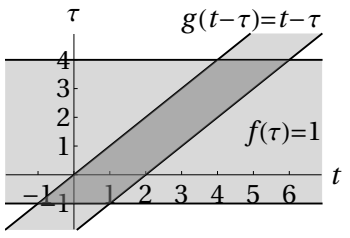
\includegraphics[width = 4.5cm]{include/Integraltransformationen/img/Faltungsgrenzen.png}
  \\\textbf{Beispiel}
  \\$f(t)= \begin{cases}
    2 \textrm{ für } 0 <t<4 \\
    0 \textrm{ sonst}
  \end{cases}
  g(t) = \begin{cases}
    3 \textrm{ für } 0<t<1 \\
    0 \textrm{ sonst}
  \end{cases}$
    \\1.$(f * g)(t) \int \limits _{-\infty} ^{\infty} f(\tau)g(t-\tau)d\tau$
    \\2.  $f(t): 0<\tau<4g(t): 0<t-\tau<1 \Rightarrow t-1 < \tau < t$
    \\3.  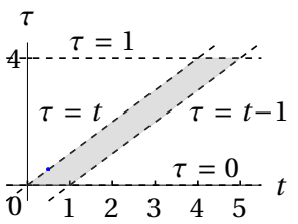
\includegraphics[width = 2cm]{include/Integraltransformationen/img/Bsp_Grenzen.png}
    \\4. und 5. $(f*g)(t) =$
    \\$t \leq 0: 0$
  \\$0 < t \leq 1: \int \limits _0 ^t 2 \cdot 3 d\tau$
    \\$1<t \leq 4: \int \limits _{t-1} ^t 2\cdot 3 d\tau$
  \\$4 <t \leq 5: \int \limits _{t-1} ^4 2\cdot 3 d\tau$
    \\$5< t: 0$

\end{multicols}


\subsection{Fourier-Reihe und Transformation}
\subsubsection*{Fourier-Reihe}
\begin{tabular}{p{4.5cm}p{11.5cm}}
  Trigonometrische Form    &
  $x(t) = \frac{a_0}{2} + \sum \limits _{n = 1} ^{\infty} a_n \cdot cos(2\pi n f_0 \cdot t) + b_n \cdot sin(2\pi n f_0 \cdot t) $
  \newline $a_n = \frac{2}{T} \int \limits _{T} x(t) dt$
  \newline $a_n = \frac{2}{T} \int \limits _{T} x(t) \cdot cos(2\pi n f_0 \cdot t)dt$
  \newline $b_n = \frac{2}{T} \int \limits _{T} x(t) \cdot sin(2\pi n f_0 \cdot t)dt$
  \\
  \rowcolor{TabularBackgroundColor}
  Harmonische Form         &
  $x(t) = r_0 + \sum \limits _{n = 1} ^{\infty} r_n \cdot cos(2\pi n f_0 \cdot t + \varpi_n)$
  \newline $r_0 = \frac{u_0}{2} = \frac{1}{T} \int  \limits _{T} x(t) dt $
  $r_n > 0 = \sqrt{u_n^2 + v_n^2}$
  $\varphi = arg(u_n - j \cdot v_n) $
  \\
  Komplexe Form            &
  $x(t) = \sum \limits _{n= -\infty} ^{\infty} c_n \cdot e^{jn2\pi f_0 \cdot t}$
  \newline $c_n =\overline{c_{-n}} = \frac{1}{T} \int \limits _{0} ^{T} x(t) \cdot e^{-j n 2 \pi f_0 \cdot t} dt$
  \newline $ 2\pi f_0$ wird auch als \textbf{Kreisfrequenz}  $\omega$ bezeichnet, \newline $f_0$ = Frequenz des Grundsignals $x(t)$.
  \\
  \rowcolor{TabularBackgroundColor}
  Umrechnung Koeffizienten &
  $c_n =\overline{c_{-n}} = \frac{a_n - jb_n}{2} (n = 0,1,2,3,..., b_0 =0)$
  \newline $a_n = 2 \cdot Re(c_n); \; b_n = -2 \cdot Im(c_n) (n = 0,1,2,3,..., b_0 =0)$ \\
\end{tabular}

\begin{multicols}{2}

  \subsubsection*{Fouriertransformation $\mathcal{F}(\omega)$}
  $$ X(\omega) = \mathcal{F}[x(t)] = \int \limits _{-\infty} ^{+\infty} x(t) \cdot e^{-j \omega t} dt $$
  $$ x(t) = \mathcal{F}^{-1}[X(\omega)] = \frac{1}{2 \pi} \int \limits _{- \infty} ^{+ \infty} X(\omega) \cdot e^{j \omega t} d\omega$$
  Rechenregeln Siehe Anhang.


  \subsubsection*{Spektraldarstellung}
  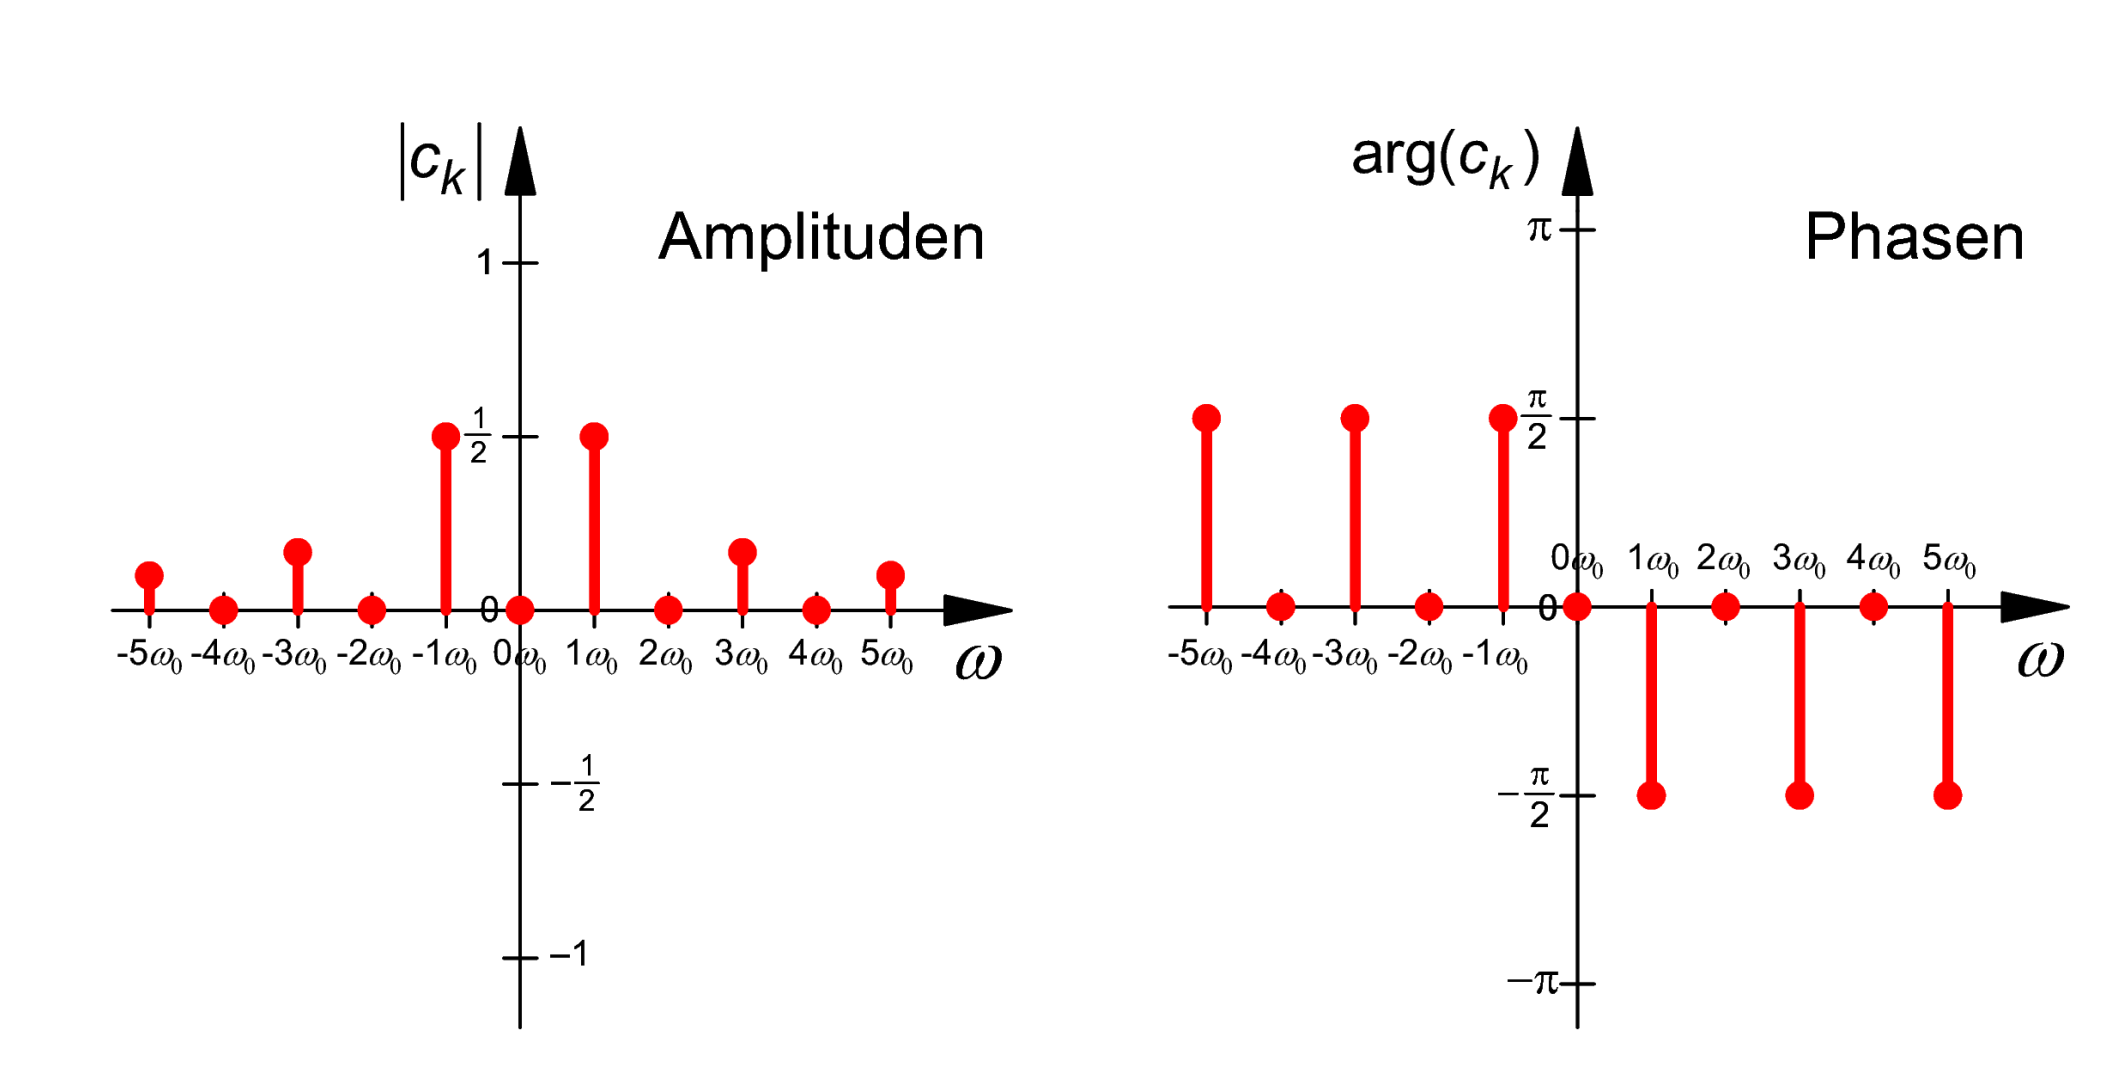
\includegraphics[width = 6cm]{include/Integraltransformationen/img/Spektrum.png}
\end{multicols}

\subsection{Laplace-Transformation}
\begin{multicols}{2}

  $$F(s) = \mathscr{L} {f(t)} = \int \limits _{0} ^{\infty} f(t) \cdot e^{-st} dt \textrm{ mit } s \in \mathbb{C}$$
  $$f(t) = \mathscr{L}^{-1} {f(t)} = \frac{1}{2\pi j} \int \limits _{p_0-j\infty} ^{p_0 + j\infty} F(s) \cdot e^{st} ds$$
  Rechenregeln Siehe Anhang.
  \subsubsection*{Lineare Differenzialgleichungen lösen:}
  DGL in Bildbereich Transformieren \\ $\Rightarrow$ DGL ist jetzt lineare Gleichung
  \\Gleichung auflösen
  \\Lösung Rücktransformieren

  \subsubsection*{Zusammenhänge}
  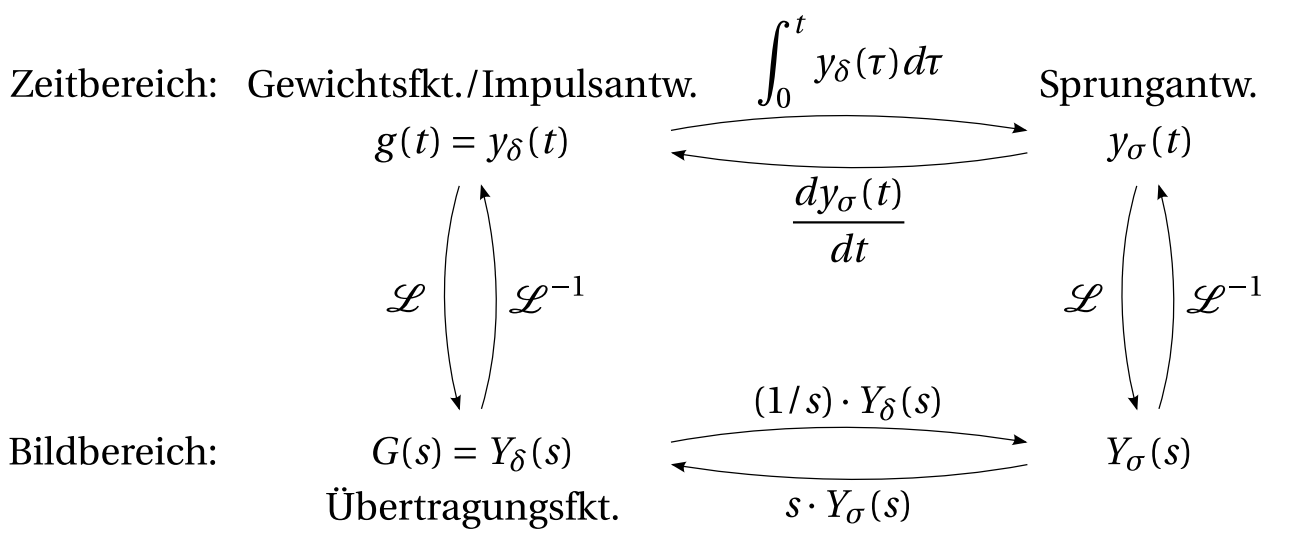
\includegraphics[width = 7cm]{include/Integraltransformationen/img/Zusammenhang_Laplace.png}

  \subsubsection*{Konvergenzhalbebene}
  Die Konvergenzhalbebene beginnt bei der Polstelle der Laplace-Transformierten mit dem Grössten Realteil und geht bis unendlich.
  \newline Bsp: Bei $\frac{1}{s-2}$ ist die Polstelle bei $+2$, daraus folgt: Konvergenzhalbebene $= [2,\infty)$
\end{multicols}

\subsection{Hilbert-Transformation}
\begin{multicols}{2}
  Im \textbf{Zeitbereich:}
  $$\hat{x}(t) = x(t) * \frac{1}{\pi t} = \frac{1}{\pi} \int \limits _{-\infty} ^{\infty} \frac{x(\tau)}{t-\tau} d\tau$$
  Im \textbf{Frequenzbereich}:
  $$\hat{X}(\omega) = X(\omega) \cdot H(\omega) = -j \cdot sgn(\omega) \cdot X(\omega)$$
\end{multicols}

%%%%%%%%%%%%%%%%%%%%%%%%%%%%%%%%%%%%%%%%%%%%%%
%Includes + Defines
%%%%%%%%%%%%%%%%%%%%%%%%%%%%%%%%%%%%%%%%%%%%%%

%\usepackage{color, colortbl}
%\usepackage{trfsigns}
%\usepackage{graphicx}
%\usepackage{adjustbox}
%\definecolor{TabularBackgroundColor}{rgb}{0.83,0.96,0.96}


%%%%%%%%%%%%%%%%%%%%%%%%%%%%%%%%%%%%%%%%%%%%%%
%Content
%%%%%%%%%%%%%%%%%%%%%%%%%%%%%%%%%%%%%%%%%%%%%%

\section{Wichtige Funktionen}

\small

\subsubsection*{Diracimpuls \tiny (auch Impuls-/Deltafunktion,-Distribution)}

\begin{multicols}{2}

  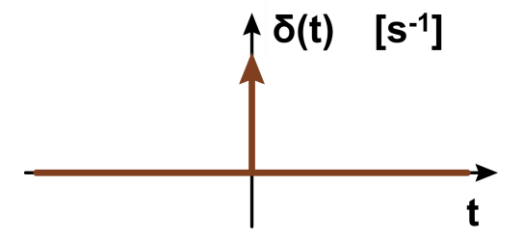
\includegraphics[width = 5cm]{include/Wichtige Funktionen/img/Impulsfunktion.png}

  {\footnotesize
    Unendlich kurzer, normierter Impuls mit unendlicher Amplitude. }

  \resizebox{0.45\textwidth}{!}{%
    \begin{tabular}{ccl}
      \hline \rowcolor{TabularBackgroundColor}
      1.  & $\delta(-t) = \delta(t) $                                                                                            & gerade Funktion                        \\
      \hline
      2.  & $\delta(-t+t_0) = \delta(t-t_0)$                                                                                     & symmetrisch                            \\
      \hline \rowcolor{TabularBackgroundColor}
      3.  & $\delta(at)= \frac{1}{|a|}\delta(t)$                                                                                 & Skalierung                             \\
      \hline
      4.  & $\delta(\frac{t-t_0}{a}) = |a| \cdot \delta(t-t_0)$                                                                  & Skalierung und Verschiebung            \\
      \hline \rowcolor{TabularBackgroundColor}
      5.  & $\delta(t-t_0)f(t) = f(t_0)\delta(t-t_0)$                                                                            & Abtastung                              \\
      \hline
      6.  & $\int \limits _{-\infty} ^{\infty} \delta(t-t_0)f(t)dt = f(t_0)$                                                     & Siebungseigenschaft                    \\
      \hline \rowcolor{TabularBackgroundColor}
      7.  & $\int \limits _{-\infty} ^{\infty}  A\cdot \delta(t)dt = A$                                                          & Spezialfall Siebungseigenschaft        \\
      \hline
      8.  & $\delta(t-t_0) * f(t) = f(t-t_0)$                                                                                    & Faltung                                \\
      \hline \rowcolor{TabularBackgroundColor}
      9.  & $\delta(t-t_1) * \delta(t-t_2) = \delta(t-t_1-t_2)$                                                                  & Faltung                                \\
      \hline
      10. & $\delta(t) = \frac{du(t)}{dt}$                                                                                       & Ableitung Einheitssprung               \\
      \hline \rowcolor{TabularBackgroundColor}
      11. & $ \delta(t) = \lim _{\omega \to \infty} \frac{sin(\omega t)}{\pi t} $                                                & Definition                             \\
      \hline
      12. & $ \delta(t) = \lim _{\epsilon \to \infty} \frac{\epsilon}{\pi(t^2 + \epsilon^2)} $                                   & Definition                             \\
      \hline \rowcolor{TabularBackgroundColor}
      13. & $\delta(t) = \lim _{\epsilon \to 0} \frac{e^{-t^2/\epsilon}}{\sqrt{(\pi \epsilon)}} $                                & Definition                             \\
      \hline
      14. & $t^n \frac{d^n \delta(t)}{dt^n} = (-1)^n n! \delta(t)$                                                               & Ableitung                              \\
      \hline \rowcolor{TabularBackgroundColor}
      15. & $f(t) * \frac{d\delta(t-t_0)}{dt} = \frac{df(t-t_0)}{dt}$                                                            & Faltung mit Ableitung                  \\
      \hline
      16. & $\frac{d\delta(t)}{dt} = \frac{\delta(t)}{-t} = \lim _{\epsilon \to 0} \frac{-2\epsilon t}{\pi(t^2 + \epsilon^2)^2}$ & 1. Ableitung $\delta(t)$ = ungerade F. \\
      \hline \rowcolor{TabularBackgroundColor}
      17. & $1$ \laplace $2\pi\delta(\omega)$                                                                                    & Fourier                                \\
      \hline
      18. & $\delta(t)$ \laplace $1(\omega)$                                                                                     & Fourier                                \\
    \end{tabular}}
\end{multicols}
\begin{tabular}{|p{3.5cm}|p{3.5cm}|p{2cm}|p{3cm}|p{3.5cm}|}
  \hline

  \textbf{Name}
   &
  \textbf{Definition}
   &
  \laplace
   &
  \textbf{Formelzeichen}
   &
  \textbf{plot}
  \\
  \hline
  Sprungfunktion
  \newline (Heaviside)
   &
  $\begin{cases}
       0 \textrm{ für }  t<0,               \\
       [\frac{1}{2} \textrm{ für }  t = 0,] \\
       1 \textrm{ für }  t >0.
     \end{cases}$
  \newline \tiny(machmal: 1 für $t=0$)
   &
  $\frac{1}{j\omega} + \pi\delta(\omega)$
   &
  $u(t), \sigma(t), h(t)$
   &
  \raisebox{-.5\height}{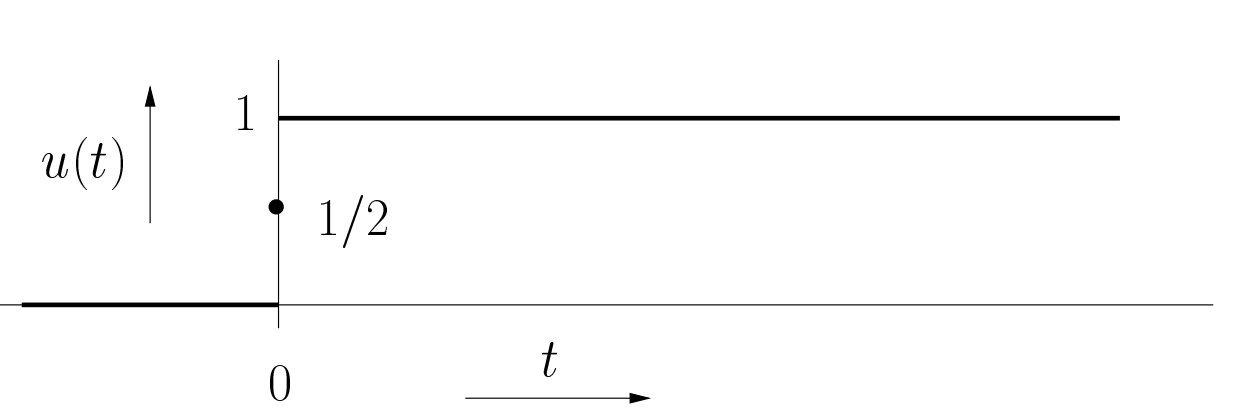
\includegraphics[width = 3.5cm]{include/Wichtige Funktionen/img/Sprungfunktion.png}}
  \\
  Signumfunktion
  \newline (Vorzeichenfunktion)
   &
  $\begin{cases}
       -1 \textrm{ für }  t<0,  \\
       0 \textrm{ für }  t = 0, \\
       1 \textrm{ für }  t >0.
     \end{cases}   $
   &
  $\frac{2}{j\omega}$
   &
  $sgn(t)$
   &
  \raisebox{-.5\height}{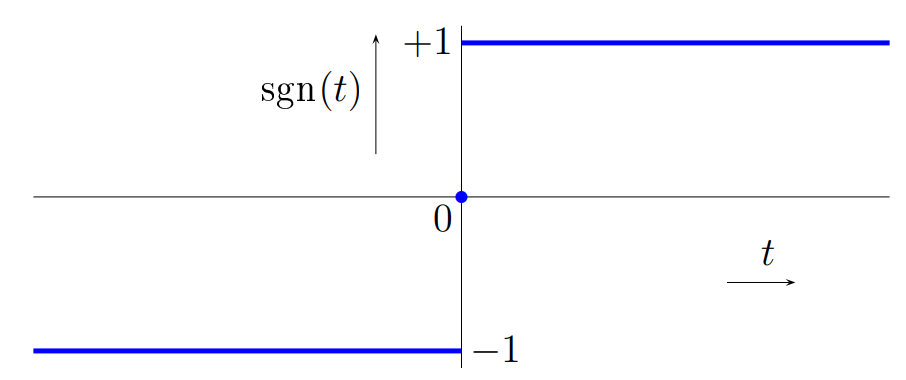
\includegraphics[width=3.5cm]{include/Wichtige Funktionen/img/Signumfunktion.png}}
  \\
  Rampenfunktion
   &
  $\begin{cases}
       0 \textrm{ für } t \leq 0, \\
       t \textrm{ für } t > 0.
     \end{cases}$
   &
  $\frac{1}{s^2}$
   &
  $r(t)$
   &
  \raisebox{-.5\height}{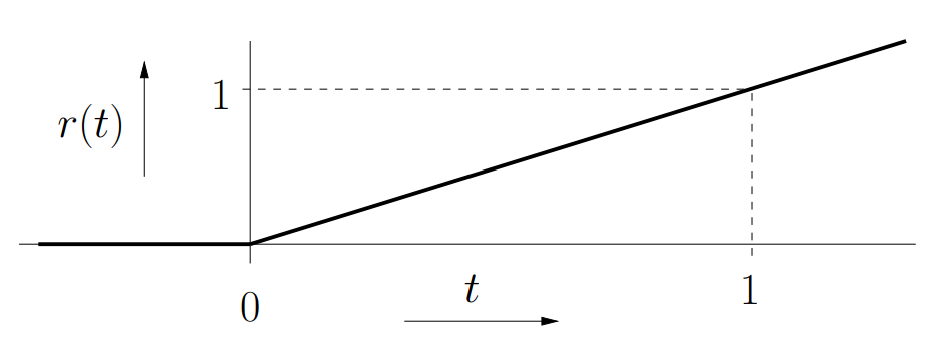
\includegraphics[width=3.5cm]{include/Wichtige Funktionen/img/Rampenfunktion.png}}
  \\
  Rechteckimpuls
   &
  $\begin{cases}
       1 \textrm{ für } |t| < a,           \\
       \frac{1}{2} \textrm{ für } |t| = a, \\
       0 \textrm{ für } |t| > a.
     \end{cases} $
   &
  $\frac{1}{s}- e^{-as}\frac{1}{s} $
   &
  $p_a(t), \beta(t)$
  \newline $\sigma(t+a)-\sigma(t-a)$
   &
  \raisebox{-.5\height}{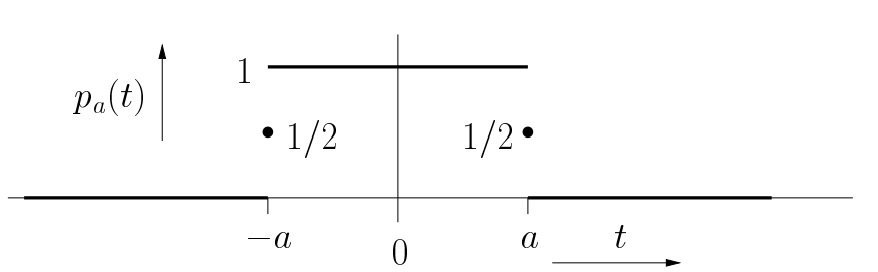
\includegraphics[width=3.5cm]{include/Wichtige Funktionen/img/Rechteckimpuls.png}}
  \\
  Dreieckimpuls
   &
  $\begin{cases}
       1 - \frac{|t|}{a} \textrm{ für } |t| < a \\
       0 \textrm{ für } |t| \geq a
     \end{cases}$
   &
  $sinc^2(\omega)$
   &
  $\Lambda(t)$
   &
  \raisebox{-.5\height}{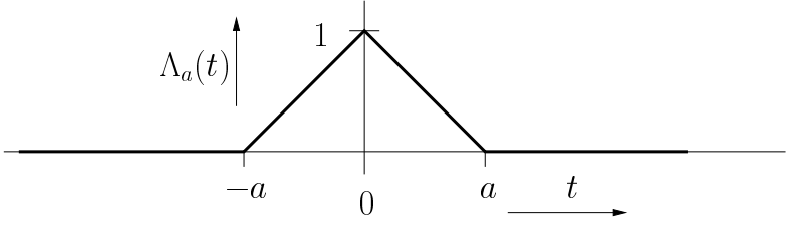
\includegraphics[width=3.5cm]{include/Wichtige Funktionen/img/Dreieckimpuls.png}}
  \\
  Sinc-Funktion
   &
  $\frac{sin(t)}{t}\; \forall t$
  \newline {\tiny $\lim _{t \to 0} sinc(t) = 1$}
  \newline {\tiny wenn normalisiert: $t \to \pi t$}
   &
  $\beta(\omega)$
  \newline{\tiny(Rechteckimpuls)}
   &
  sinc(t)
   &
  \raisebox{-.5\height}{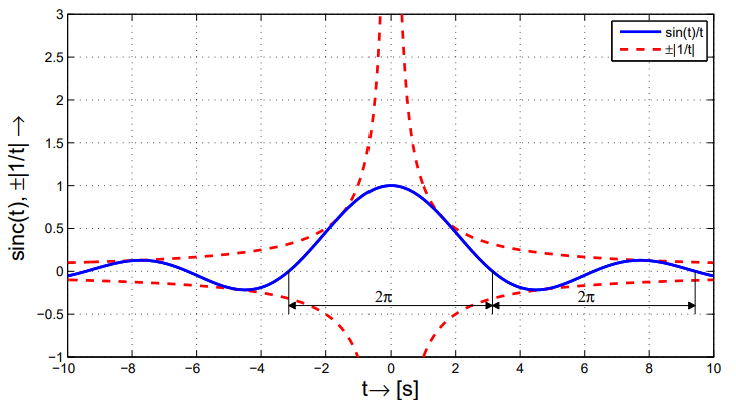
\includegraphics[width=3.5cm]{include/Wichtige Funktionen/img/SincFunktion.png}}
  \\
  \hline
\end{tabular}

% Needs Package: 
%\usepackage{bm}
%\usepackage{multicol}
\section{LTI-Systeme}

$ y(t) = \mathcal{T}[x(t)]$

\begin{multicols}{2}
    \subsection*{Linearität und Zeitinvarianz}
    \begin{itemize}
        \item $\mathcal{T}[x_1(t) + x_2(t)] = y_1(t) + y_2(t)$
        \item $\mathcal{T}[k_a \cdot x(t)] = k_a \cdot y(t)$
        \item $\mathcal{T}[x(t-t_0) = y(t-t_0)]$
    \end{itemize}

    \subsection{Beschreibung von LTI Systemen}

    \subsubsection{Impulsantwort}
    Impulsfunktion $\delta(t)$ wird am Eingang des Systems angelegt,
    die Reaktion darauf am Ausgang nennt man die \textbf{Impulsantwort} \bm{$h(t)$}.
    Sie beschreibt ein LTI-System vollständig.

    $$ y(t) = \mathcal{T}[x(t)]
        = \int \limits _{-\infty} ^{\infty} x(\tau) \cdot h(t-\tau)d\tau
        = x(t) * h(t)$$
  
    \subsubsection{Frequenzantwort}
    Die \textbf{Frequenzantwort} $\bm{H(\omega)}$ ist die Fouriertransformierte Impulsantwort.
    Sie ist eine komplexwertige dimensionslose Gewichstsfunktion.
    Auch sie beschreibt ein LTI-System vollständig.

    $$ Y(\omega) = X(\omega) \cdot H(\omega)$$

    \subsubsection{Berechnung des Ausgangssignals}
\begin{enumerate}
   \item Fourier-Transformation:  $X(\omega) = \mathcal{F}[x(t)]$ 
   \item Berechnung in Frequenz  $Y(\omega) = X(\omega) \cdot H(\omega)$ 
   \item Rücktransformation:  $y(t) = \mathcal{F}^{-1}[Y(\omega)]$ 
\end{enumerate}


    \subsection{Bezeichnungen}
    Übertragungsfunktion: $H(\omega)=|H(\omega)| \cdot e^{j\varphi_H(\omega)}$ \\
    Amplitudengang: $|H(\omega)|$ \\
    Phasengang: $\varphi_H(\omega)$ \\

    \subsubsection{Filtereigenschaften}
    $Y(\omega) = X(\omega) \cdot H(\omega)$ \\
    $|Y(\omega)| = |X(\omega)| \cdot |H(\omega)|$ \\
    $\varphi_y(\omega) = \varphi_x(\omega) + \varphi_H(\varphi)$

\end{multicols}

%%%%%%%%%%%%%%%%%%%%%%%%%%%%%%%%%%%%%%%%%%%%%%
%Includes + Defines
%%%%%%%%%%%%%%%%%%%%%%%%%%%%%%%%%%%%%%%%%%%%%%

%\usepackage{color, colortbl}
%\usepackage{trfsigns}
%\usepackage{graphicx}
%\definecolor{TabularBackgroundColor}{rgb}{0.83,0.96,0.96}


%%%%%%%%%%%%%%%%%%%%%%%%%%%%%%%%%%%%%%%%%%%%%%
%Content
%%%%%%%%%%%%%%%%%%%%%%%%%%%%%%%%%%%%%%%%%%%%%%


\subsection{Integrieren und Differenzieren}
\subsubsection{Integrationsregeln}
\begin{tabular}{ll}
  Linearit\"at                    & $\int{f(\alpha x+\beta )dx=\frac{1}{\alpha}\cdot F(\alpha x+\beta)+C}$ \\
  
  \rowcolor{TabularBackgroundColor}
  Partielle Integration           & $\int\limits_a^b{u'(x)\cdot v(x)dx}=\biggl[
      u(x)\cdot v(x) \biggr]_a^b-\int\limits_a^b{u(x)\cdot v'(x)dx}$
  \tiny($v(x)$ = einfacheste Funktion wählen!) \normalsize                                                 \\

  Substitution (Rationalisierung) & $t=\tan\frac{x}{2}, \qquad
    dx=\frac{2dt}{1+t^2} \qquad \sin  x=\frac{2t}{1+t^2} \qquad \cos x=\frac{1-t^2}{1+t^2}
  \quad\int{R(\sin(x)\cos(x))dx}$                                                                          \\
  
  \rowcolor{TabularBackgroundColor}
  Allgemeine Substitution         &
  $\int\limits_{a}^{b}{f(x)dx}=\int\limits_{g(a)}^{g(b)}{f(g(t))\cdot
  g'(t)dt}\qquad x=g(t)\qquad g'(t)=\frac{dt}{dx}\qquad dx=\frac{1}{g'(t)}\cdot dt$                        \\

  Logarithmische Integration      & $\int{\frac{f'(x)}{f(x)}dx}=\ln|f(x)|+C
  \qquad{(f(x)\neq 1)}$                                                                                    \\

  \rowcolor{TabularBackgroundColor}
  Spezielle Form des Integranden  & $\int{f'(x)\cdot
      (f(x))^{\alpha} dx}= f(x)^{\alpha +1}\cdot \frac{1}{\alpha+1}+C
  \qquad{(\alpha \neq -1)}$                                                                                \\

  Differentiation                 & $\int \limits ^{b} _{a} {f'(t)dt}=f(b)-f(a)$\qquad
  $\frac{d}{dx} \int \limits ^{x} _{1} {f(t)dt}=f(x)$
\end{tabular}
\\

\begin{minipage}{0.5\textwidth}
  \subsubsection{Ableitungsregeln}
  \begin{tabular}{ll}
    Linerität       & $(\lambda f + \mu g)'(x) = \lambda f'(x) + \mu g'(x)$ \\
    \rowcolor{TabularBackgroundColor}
    Produktregel    & $(f\cdot g)' = f'g + fg'$                             \\
    Quotientenregel & $(\frac{f}{g})' = \frac{f'g - fg'}{g^2}$              \\
    \rowcolor{TabularBackgroundColor}
    Kettenregel     & $ (f(g))' = f'(g) \cdot g' $                          \\
    Potenz          & $((x-a)^n)'= n\cdot(x-a)^{n-1}$                       \\
    \rowcolor{TabularBackgroundColor}
    Trigo           & $sin'' = cos' = -sin$                                 \\
    Schrittfunktion & $\sigma'(t) = \delta(t)$
  \end{tabular}
\end{minipage}%
\begin{minipage}{0.5\textwidth}
  \subsection{Partialbruchzerlegung}
  Nenner Faktorisieren (Nennerexponent)
  \\Zähler = Polynom (Nennergrad -1)
  \\Gleichsetzen mit Originalbruch
  \\Mit Gleichungssystem auflösen.
  \\Ansätze:
  \\ $\frac{\dots}{x(x-3)^2} = \frac{A}{x} + \frac{B}{x-3} + \frac{C}{(x-3)^2}$
  \\ $\frac{\dots}{(x-2)^3} = \frac{A}{x-2} + \frac{B}{(x-2)^2} + \frac{C}{(x-2)^3}$
  \\ $\frac{\dots}{x^4 + x^2} = \frac{A}{x} + \frac{B}{x^2} + \frac{Cx + D}{x^2 + 1}$
\end{minipage}

\section*{Wichtige Werte \& Vereinfachungen}

\subsubsection*{Integration über Periodendauer}
$$\int_T (x \cdot sin(\omega t + \alpha))^2 dt = x^2 \cdot \int_T sin^2(\omega t +\alpha) dt = \frac{x^2}{2}$$
$$\int_T (x \cdot cos(\omega t+\alpha))^2 dt = x^2 \cdot \int_T cos^2(\omega t+\alpha) dt = \frac{x^2}{2}$$


\subsubsection*{Komplex sin/cos}

$$cos \varphi = \frac{e^{j\varphi}+ e^{-j\varphi}}{2}, \; sin \varphi = \frac{e^{j\varphi} - e^{-j\varphi}}{2j} $$




\newpage
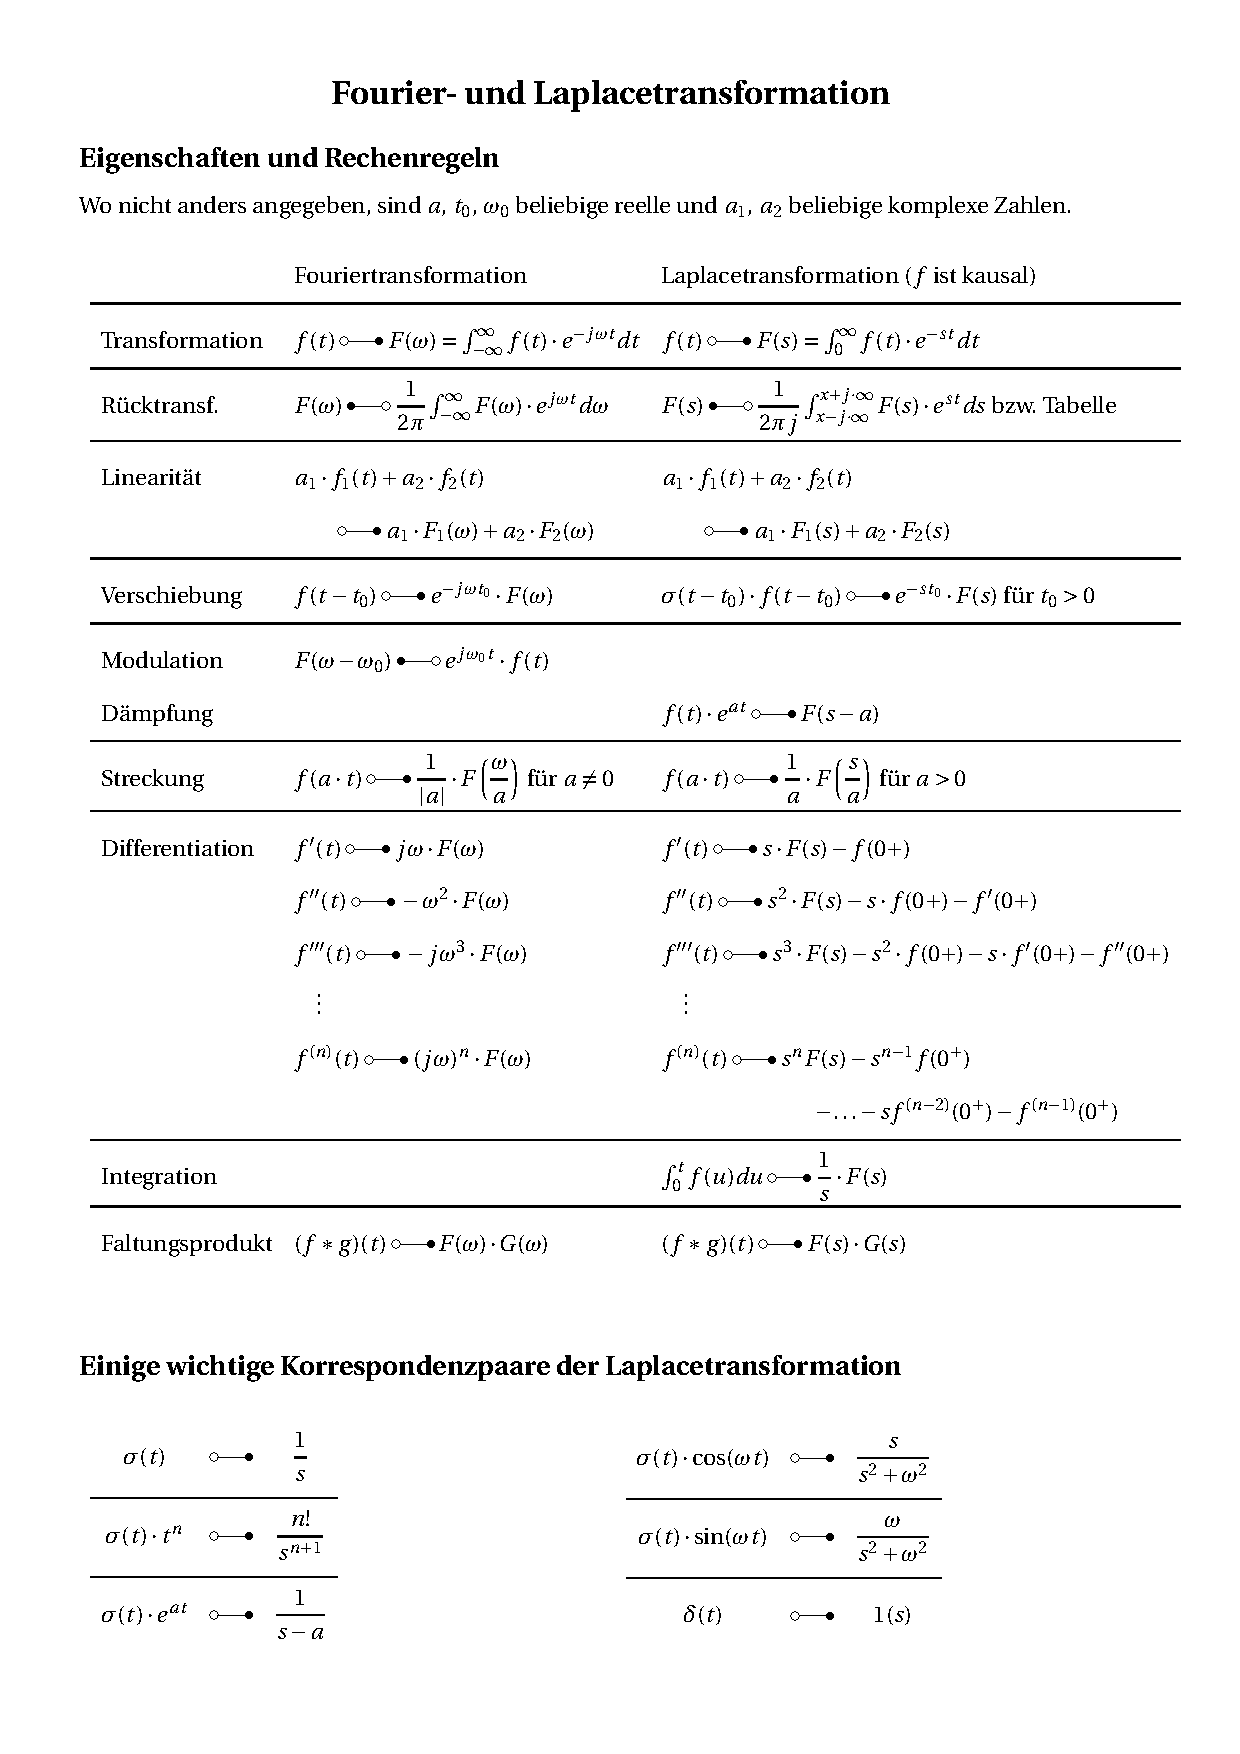
\includepdf[pages=-]{AnhangPDF/fourierLaplaceTabelle_v02.pdf}

\end{document}
